\documentclass[10pt]{article}
\usepackage[provide=*,spanish]{babel}
\usepackage{fontspec}
\defaultfontfeatures{Ligatures=TeX}
\setmainfont{Latin Modern Roman}
\setsansfont{Latin Modern Sans}
\setmonofont{Latin Modern Mono}
\usepackage[a4paper,margin=2.25cm,headheight=15pt]{geometry}
\usepackage{amsmath,amssymb}
\usepackage{booktabs,longtable,tabularx,array}
\usepackage{graphicx,float}
\usepackage{xcolor}
\usepackage{hyperref}

\definecolor{uvgverde}{HTML}{176B52}
\definecolor{uvgoscuro}{HTML}{103F33}
\definecolor{grisclaro}{HTML}{F2F5F4}
\definecolor{azulcli}{HTML}{17324D}
\hypersetup{colorlinks=true,linkcolor=uvgoscuro,urlcolor=uvgverde,pdfauthor={Grupo 1 - CC3067},pdftitle={Laboratorio 3 - Algoritmos de Enrutamiento}}

\pagestyle{plain}
\renewcommand{\arraystretch}{1.18}

\newcolumntype{Y}{>{\raggedright\arraybackslash}X}
\newcolumntype{C}[1]{>{\centering\arraybackslash}p{#1}}
\newenvironment{calculo}[1][]{\par\medskip\noindent\color{uvgoscuro}\hrule\smallskip\textbf{Desarrollo del calculo}\par\color{black}}{\par\smallskip\color{uvgoscuro}\hrule\color{black}\medskip}
\newenvironment{decision}[1][]{\par\medskip\noindent\color{uvgoscuro}\hrule\smallskip\textbf{Decision de diseno}\par\color{black}}{\par\smallskip\color{uvgoscuro}\hrule\color{black}\medskip}
\newenvironment{evidencia}[1][]{\par\medskip\noindent\color{azulcli}\hrule\smallskip\textbf{Evidencia real de Packet Tracer}\par\color{black}}{\par\smallskip\color{azulcli}\hrule\color{black}\medskip}

\newcommand{\universidad}{Universidad del Valle de Guatemala}
\newcommand{\curso}{CC3067 Redes}
\newcommand{\seccion}{Seccion 10}
\newcommand{\grupo}{Grupo 1}
\newcommand{\integrantes}{%
\begin{tabular}{ll}
Pablo Daniel Barillas Moreno & 22193\\
Andres Rafael Chivalan & 21534
\end{tabular}}

\newcommand{\portadalab}[2]{%
\begin{titlepage}
\centering
{\Large\bfseries \universidad\par}
\vspace{1.2cm}
{\large \curso\ -- \seccion\par}
\vspace{2.2cm}
{\Huge\bfseries Laboratorio 3\par}
\vspace{0.35cm}
{\LARGE Algoritmos de Enrutamiento\par}
\vspace{0.8cm}
{\Large\color{uvgverde}#1\par}
\vfill
{\large\bfseries \grupo\par}
\vspace{0.45cm}
\integrantes
\vfill
{\large #2\par}
\end{titlepage}}



\begin{document}
\portadalab{PDF 2: evidencias reales de Packet Tracer}{5 de octubre de 2026}
\tableofcontents
\newpage

\section{Metodologia de evidencia}

Las salidas de este documento fueron leidas directamente de los dispositivos de la topologia guardada. No son resultados esperados escritos antes de la prueba. Primero se verificaron enlaces e IP, luego adyacencias, tablas de enrutamiento, ECMP, DUAL, pings y trazas.

\begin{evidencia}
Estado de salud del proyecto: cero enlaces caidos y cero direcciones IP duplicadas. Los seis pings representativos terminaron con cuatro respuestas de cuatro intentos.
\end{evidencia}

\section{Topologia implementada}
\begin{figure}[H]
\centering
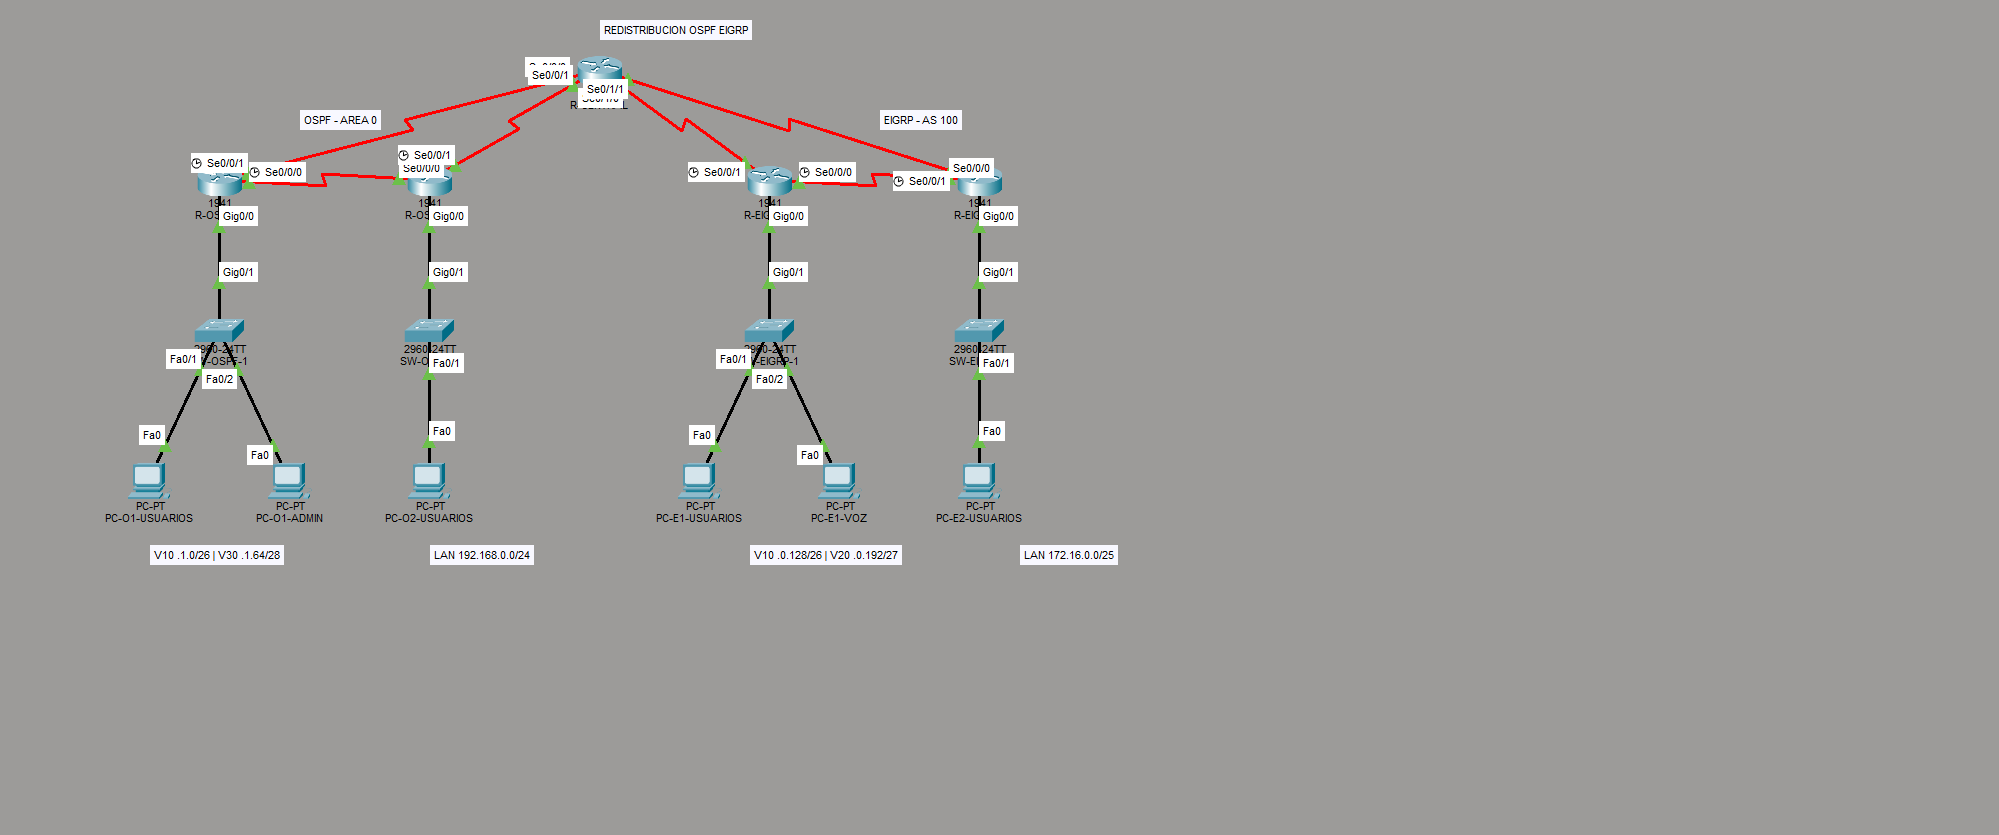
\includegraphics[width=\textwidth,trim=80 175 650 15,clip]{figuras/topologia_lab3.png}
\caption{Topologia real construida: cinco routers, seis enlaces seriales, cuatro switches y seis hosts de prueba.}
\end{figure}

Los enlaces seriales forman dos triangulos que comparten R-CENTRAL. R-OSPF-1 y R-EIGRP-1 usan router-on-a-stick. El central no tiene LAN y es el unico router con ambos protocolos.

\section{Resumen de interfaces y gateways}
\small
\begin{longtable}{p{2.6cm}p{3.0cm}p{3.1cm}p{4.6cm}}
\toprule
Equipo & Interfaz & IP/prefijo & Funcion\\
\midrule
\endhead
R-OSPF-1 & G0/0.10 & 192.168.1.1/26 & Gateway VLAN 10\\
R-OSPF-1 & G0/0.30 & 192.168.1.65/28 & Gateway VLAN 30\\
R-OSPF-1 & S0/0/0, S0/0/1 & 10.0.0.1/30, 10.0.0.5/30 & Directo y central\\
R-OSPF-2 & G0/0 & 192.168.0.1/24 & Gateway LAN 200 hosts\\
R-OSPF-2 & S0/0/0, S0/0/1 & 10.0.0.2/30, 10.0.0.9/30 & Directo y central\\
R-CENTRAL & S0/0/0, S0/0/1 & 10.0.0.6/30, 10.0.0.10/30 & Lado OSPF\\
R-CENTRAL & S0/1/0, S0/1/1 & 10.0.0.18/30, 10.0.0.22/30 & Lado EIGRP\\
R-EIGRP-1 & G0/0.10, G0/0.20 & 172.16.0.129/26, 172.16.0.193/27 & Gateways VLAN 10 y 20\\
R-EIGRP-1 & S0/0/0, S0/0/1 & 10.0.0.13/30, 10.0.0.17/30 & Directo y central\\
R-EIGRP-2 & G0/0 & 172.16.0.1/25 & Gateway LAN 100 hosts\\
R-EIGRP-2 & S0/0/0, S0/0/1 & 10.0.0.14/30, 10.0.0.21/30 & Directo y central\\
\bottomrule
\end{longtable}
\normalsize

\section{Tablas de enrutamiento de los cinco routers}

Para evitar que el paginador de la consola oculte lineas, la tabla se consulto por origen con \texttt{show ip route connected}, \texttt{show ip route ospf} y \texttt{show ip route eigrp}. En conjunto equivalen a la tabla completa y permiten distinguir el origen de cada ruta.

\subsection{R-OSPF-1}
\begin{verbatim}
C 10.0.0.0/30       is directly connected, Serial0/0/0
C 10.0.0.4/30       is directly connected, Serial0/0/1
C 192.168.1.0/26    is directly connected, GigabitEthernet0/0.10
C 192.168.1.64/28   is directly connected, GigabitEthernet0/0.30
O 192.168.0.0/24 [110/21] via 10.0.0.2, Serial0/0/0
                   [110/21] via 10.0.0.6, Serial0/0/1
O E1 172.16.0.0/25   [110/30] via 10.0.0.6, Serial0/0/1
O E1 172.16.0.128/26 [110/30] via 10.0.0.6, Serial0/0/1
O E1 172.16.0.192/27 [110/30] via 10.0.0.6, Serial0/0/1
\end{verbatim}

\subsection{R-OSPF-2}
\begin{verbatim}
C 10.0.0.0/30    is directly connected, Serial0/0/0
C 10.0.0.8/30    is directly connected, Serial0/0/1
C 192.168.0.0/24 is directly connected, GigabitEthernet0/0
O 192.168.1.0/26 [110/21] via 10.0.0.1, Serial0/0/0
                  [110/21] via 10.0.0.10, Serial0/0/1
O 192.168.1.64/28 [110/21] via 10.0.0.1, Serial0/0/0
                   [110/21] via 10.0.0.10, Serial0/0/1
O E1 172.16.0.0/25   [110/30] via 10.0.0.10, Serial0/0/1
O E1 172.16.0.128/26 [110/30] via 10.0.0.10, Serial0/0/1
O E1 172.16.0.192/27 [110/30] via 10.0.0.10, Serial0/0/1
\end{verbatim}

\subsection{R-CENTRAL}
\begin{verbatim}
C 10.0.0.4/30  is directly connected, Serial0/0/0
C 10.0.0.8/30  is directly connected, Serial0/0/1
C 10.0.0.16/30 is directly connected, Serial0/1/0
C 10.0.0.20/30 is directly connected, Serial0/1/1
O 192.168.0.0/24  [110/11] via 10.0.0.9, Serial0/0/1
O 192.168.1.0/26  [110/11] via 10.0.0.5, Serial0/0/0
O 192.168.1.64/28 [110/11] via 10.0.0.5, Serial0/0/0
D 172.16.0.0/25   [90/1683712] via 10.0.0.21, Serial0/1/1
D 172.16.0.128/26 [90/1686016] via 10.0.0.17, Serial0/1/0
D 172.16.0.192/27 [90/1686016] via 10.0.0.17, Serial0/1/0
D 192.168.0.0/23 is a summary, Null0
\end{verbatim}

\subsection{R-EIGRP-1}
\begin{verbatim}
C 10.0.0.12/30     is directly connected, Serial0/0/0
C 10.0.0.16/30     is directly connected, Serial0/0/1
C 172.16.0.128/26  is directly connected, GigabitEthernet0/0.10
C 172.16.0.192/27  is directly connected, GigabitEthernet0/0.20
D 172.16.0.0/25 [90/2170112] via 10.0.0.14, Serial0/0/0
                 [90/6510336] via 10.0.0.18, Serial0/0/1
D 192.168.0.0/23 [90/6996480] via 10.0.0.18, Serial0/0/1
\end{verbatim}

\subsection{R-EIGRP-2}
\begin{verbatim}
C 10.0.0.12/30  is directly connected, Serial0/0/0
C 10.0.0.20/30  is directly connected, Serial0/0/1
C 172.16.0.0/25 is directly connected, GigabitEthernet0/0
D 172.16.0.128/26 [90/2172416] via 10.0.0.13, Serial0/0/0
                   [90/6512640] via 10.0.0.22, Serial0/0/1
D 172.16.0.192/27 [90/2172416] via 10.0.0.13, Serial0/0/0
                   [90/6512640] via 10.0.0.22, Serial0/0/1
D 192.168.0.0/23 [90/6996480] via 10.0.0.22, Serial0/0/1
\end{verbatim}

\section{Evidencia OSPF de costo igual}

\begin{evidencia}[title={Comando: show ip route 192.168.0.0 en R-OSPF-1}]
\begin{verbatim}
Routing entry for 192.168.0.0/24
Known via "ospf 1", distance 110, metric 21, type intra area
  Routing Descriptor Blocks:
  * 10.0.0.2, from 2.2.2.2, via Serial0/0/0
      Route metric is 21, traffic share count is 1
    10.0.0.6, from 2.2.2.2, via Serial0/0/1
      Route metric is 21, traffic share count is 1
\end{verbatim}
\end{evidencia}

Los dos siguientes saltos tienen metrica 21. El primero usa el enlace directo y el segundo pasa por R-CENTRAL. \texttt{show ip ospf interface} se conserva como comprobacion de costos de interfaz; la presencia de los dos siguientes saltos se demuestra con \texttt{show ip route}, que es el comando que realmente lista las rutas instaladas.

\section{Evidencia EIGRP 75/25 y condicion de factibilidad}

\begin{evidencia}[title={Comando: show ip eigrp topology 172.16.0.0 255.255.255.128}]
\begin{verbatim}
IP-EIGRP (AS 100): Topology entry for 172.16.0.0/25
  State is Passive, 2 Successor(s), FD is 2170112
  Routing Descriptor Blocks:
  10.0.0.14 (Serial0/0/0)
      Composite metric is (2170112/2816), Route is Internal
      Total delay is 20010 microseconds
  10.0.0.18 (Serial0/0/1)
      Composite metric is (6510336/1683712), Route is Internal
      Total delay is 189550 microseconds
\end{verbatim}
\end{evidencia}

Antes de aplicar \texttt{variance}, el camino directo es el sucesor y el camino por el central es sucesor factible porque $1\,683\,712<2\,170\,112$. Con \texttt{variance 3} ambos se instalan; la relacion de metricas es exactamente $3:1$, de donde se obtiene el reparto aproximado 75/25.

\section{Redistribucion y resumen}

\begin{evidencia}[title={Ruta resumida vista desde ambos routers EIGRP}]
\begin{verbatim}
R-EIGRP-1# show ip route 192.168.0.0 255.255.254.0
Known via "eigrp 100", distance 90, metric 6996480
* 10.0.0.18, via Serial0/0/1

R-EIGRP-2# show ip route 192.168.0.0 255.255.254.0
Known via "eigrp 100", distance 90, metric 6996480
* 10.0.0.22, via Serial0/0/1
\end{verbatim}
\end{evidencia}

Las redes del otro dominio aparecen como OSPF E1, lo que demuestra la redistribucion desde EIGRP hacia OSPF. En sentido opuesto, la metrica semilla EIGRP configurada fue \texttt{1544 20000 255 1 1500}. La ruta OSPF se anuncia al lado EIGRP como el resumen \texttt{192.168.0.0/23}.

El IOS emulado no admite route-maps ni \texttt{summary-address} dentro de OSPF. Por ello la salida OSPF conserva los tres prefijos EIGRP especificos y tambien muestra los /30 redistribuidos. Esta limitacion se verifico en la CLI y se declara expresamente; no se atribuye al equipo una funcion que el simulador rechazo.

\section{Pruebas de conectividad}

Despues de resolver ARP con una primera prueba, la matriz final fue:

\begin{center}
\begin{tabularx}{\textwidth}{Y l C{1.8cm} C{2cm}}
\toprule
Origen & Destino & Recibidos & Perdida\\
\midrule
PC-O1-USUARIOS & 172.16.0.2 & 4/4 & 0\%\\
PC-O1-ADMIN & 172.16.0.194 & 4/4 & 0\%\\
PC-O2-USUARIOS & 172.16.0.130 & 4/4 & 0\%\\
PC-E1-USUARIOS & 192.168.0.2 & 4/4 & 0\%\\
PC-E1-VOZ & 192.168.1.66 & 4/4 & 0\%\\
PC-E2-USUARIOS & 192.168.1.2 & 4/4 & 0\%\\
\bottomrule
\end{tabularx}
\end{center}

\subsection{Traza OSPF hacia EIGRP}
\begin{verbatim}
C:\>tracert 172.16.0.2
Tracing route to 172.16.0.2 over a maximum of 30 hops:
  1   0 ms   0 ms   0 ms   192.168.1.1
  2   1 ms   1 ms   0 ms   10.0.0.6
  3   0 ms   2 ms   3 ms   10.0.0.21
  4  11 ms  12 ms  10 ms   172.16.0.2
Trace complete.
\end{verbatim}

\subsection{Traza EIGRP hacia OSPF}
\begin{verbatim}
C:\>tracert 192.168.1.66
Tracing route to 192.168.1.66 over a maximum of 30 hops:
  1   0 ms   0 ms   0 ms   172.16.0.1
  2   1 ms  11 ms  16 ms   10.0.0.22
  3  23 ms  10 ms  10 ms   10.0.0.5
  4  34 ms  13 ms  15 ms   192.168.1.66
Trace complete.
\end{verbatim}

\section{Conclusion de verificacion}

La topologia satisface conectividad extremo a extremo entre las seis LAN/VLAN. OSPF mantiene dos caminos de costo igual; EIGRP cumple la condicion de factibilidad e instala dos rutas con relacion de metrica 3:1; R-CENTRAL realiza redistribucion mutua y el lado EIGRP recibe un solo resumen OSPF /23.

\end{document}


